\documentclass[letterpaper,10pt,titlepage,draftclsnofoot,onecolumn,compsoc,utf8,latin1]{IEEEtran}
\usepackage{graphicx}
\usepackage{amssymb}
\usepackage{amsmath}
\usepackage{array}
\usepackage{amsthm}
\usepackage{listings}
\usepackage{alltt}
\usepackage{float}
\usepackage{color}
\usepackage{url}
\usepackage{setspace}
\usepackage{balance}
\usepackage[TABBOTCAP, tight]{subfigure}
\usepackage{enumitem}
\usepackage{pstricks, pst-node}
\usepackage[utf8]{inputenc}
\usepackage[margin=.75in]{geometry}
\usepackage{titlesec}
\usepackage{fancyhdr}
\usepackage{hyperref}
\usepackage{geometry}
\usepackage{tocloft}

%hide toc subsubsections
\setcounter{tocdepth}{2}

%toc formatting for IEEE 830-1998 standards
\renewcommand{\cftsecleader}{\cftdotfill{\cftdotsep}{\vspace{.25cm}}}
\renewcommand{\cftsecfont}{\normalfont}
\renewcommand{\cftsecpagefont}{\normalfont}
\renewcommand{\cftsecaftersnum}{.}

%bottom right page numbers
\fancyhf{}
\renewcommand{\headrulewidth}{0pt}
\rfoot{\thepage}
\pagestyle{fancy}

%formatting specific IEEE 830-1998 Section headings
\titleformat{\section}[block]
  {\fontsize{12}{15}\bfseries\sffamily}
  {\thesection.}
  {1em}
  {}
\titleformat{\subsection}[block]
  {\fontsize{10}{10}\bfseries\sffamily}
  {\thesubsection}
  {1em}
  {\vspace{.1cm}}
\titleformat{\subsubsection}[block]
  {\fontsize{10}{10}\bfseries\sffamily}
  {\thesubsubsection}
  {1em}
  {\vspace{.2cm}}
\geometry{textheight=8.5in, textwidth=6in}

\newcommand{\cred}[1]{{\color{red}#1}}
\newcommand{\cblue}[1]{{\color{blue}#1}}

\def\name{Charles Siebert, Branden Berlin, Yipeng "Roger" Song}

%% The following metadata will show up in the PDF properties
\hypersetup{
  urlcolor = black,
  pdfauthor = {\name},
  pdfkeywords = {cs461 ``Senior Capstone - Fall 2016'' capstone},
  pdftitle = {CS 461 Requirements Document},
  pdfsubject = {Capstone Requirements Document},
  pdfpagemode = UseNone
}

\begin{document}
\begin{titlepage}
\centering
\vspace*{6cm}
{\scshape\LARGE \begin{singlespace}Optimizing Virtual Reality and Augmented Reality Performance on Mobile Web Applications \\ \end{singlespace} Requirements Document } \\
	{\scshape\Large CS461 - Fall 2016 \par}
	\vspace{.5cm}
	\name \par
    {\large \today \par} 
	\vspace*{1cm}
	
\begin{abstract}
The technology of Virtual Reality (VR) currently is not cost effective to today's market, as the cost of high-end setups required makes it difficult to afford. Browser developers are focusing primarily on expensive high-end high-performance hardware over mobile devices for Augmented Reality (AR) or Virtual Reality (VR) on the web. Doing AR/VR on the mobile web allows more developers to enter the field and deliver to more customers. To accomplish this, we are working on a project called “Mobile AR/VR Performance”, which focuses on researching to profile and identify performance bottlenecks in 3D web content on mobile devices. We will file issues in the open source projects for Chrome, Firefox through A-Frame and Three.js to determine and identify those bottlenecks. We hope to accomplish this by reporting the challenges and opportunities for performance VR/AR applications, and write a blog post detailing the project results and their best-practices.
\end{abstract}

\end{titlepage}

\newpage

\tableofcontents

%removes page number on table of contents
\thispagestyle{empty}

\newpage

\section{Introduction}
\begin{singlespace}
\noindent
This project requirements document outlines the entirety of the project, including the necessary definitions and references used throughout the project's duration as well as within the documents created in the project. This paper focuses on what the project is, it's purpose, and the problem it is trying to solve. The problem we need to solve is to optimize performance issues found within the A-Frame web framework, and determine how well it works on mobile devices. The software we develop for this project will be used as a series of test cases to measure the performance differences between different types of implementations, or specific scenarios in implementation where we mean to pin point bottlenecks that would occur within mobile devices. After collecting the necessary data (frame rate, processing consumption, memory consumption, battery life-span, and hardware limitations), we will compile a report that analyzes the information to determine the best practices, or bugs that may occur during development. The software we are developing will be conducted on a Nexus 5X phone, which is the standard of phone being used by other developers working on A-Frame. This helps to eliminate the possibility of hardware differences when measuring the metrics of performance data and bug-specific problems relating to hardware.
\end{singlespace}

\subsection{Purpose}
\begin{singlespace}
\noindent
The purpose of this project is to determine areas of development within A-Frame where practices will be best used, as they will least be likely to impede on bottle necking either the software or hardware whe n optimizing the software for performance. This project is focused towards the advancement of an open-source, developing web framework, and the developers making their own products with A-Frame and for mobile devices. The developers will be using our project research as a means to avoid these bottlenecks in this evolving environment.
\end{singlespace}

\subsection{Scope}
\begin{singlespace}
\noindent
Optimizing VR and AR for Mobile Web Apps is to determine Virtual Reality (VR) and Augmented Reality (AR) bottlenecks that exist in mobile devices within the A-Frame framework. The bottlenecks can be caused from either unoptimized development of software, underpowered or unoptimized hardware found in existing devices, or potential bugs or limitations found within the framework itself. The software itself, which is developed on A-Frame, will generate multiple scenes where it will test the graphical capabilities of the hardware within the mobile devices, the types of different implementations of certain scenes, and determine areas of optimization through these multiple scenes. The software will be used to create a report that will analyze the information collected about processing power, frame rates, battery usage, and the limitations of the framework to determine the best practices for implementing more graphically intensive programs on A-Frame. \\

\noindent
Developers other than us will use the information in the report to determine the best way to approach at designing their programs, as the software we create will only serve as test cases and stress testing for mobile devices to collect this information. 
\end{singlespace}

\subsection{Glossary}
\begin{singlespace}
\begin{enumerate}[labelsep=2em,leftmargin=.5in]
    {\item \bfseries Virtual Reality (VR): } Computer generated three-dimensional environment that immerses the user into the environment using special equipment or implementation techniques. \vspace{.1cm}
    {\item \bfseries Augmented Reality (AR): } Provides a composite view to the user based on computer generated environments super-imposed onto the view of the real world. \vspace{.1cm}
    {\item \bfseries Operating System (OS): } Software that supports an interface to support computer's basic functions, such as process scheduling, executing tasks, and allowing user interface. Specifically this project is in regards to Android OS. \vspace{.1cm}
    {\item \bfseries Web Framework: } A software framework that is designed to support the development of web applications including web services, web resources and web APIs. \vspace{.1cm}
    {\item \bfseries A-Frame: } A-Frame is an open-source WebVR framework for creating virtual reality (VR) experiences with HTML with the use of the Three.js framework.\vspace{.1cm}
    {\item \bfseries Three.js: } JavaScript framework that allows accessible development WebGL applications. \vspace{.1cm}
    {\item \bfseries WebGL: } JavaScript API that allows for rendering interactive 3D and 2D computer graphics within any compatible web browser without the use of plug-ins. \vspace{.1cm}
    {\item \bfseries Viewport: } A viewport is a viewing region in computer graphics. This region is defined in the software to allow for viewing the drawing of objects. This viewport is typically bounded by a window or by the full screen of the mobile device. \vspace{.1cm}
    {\item \bfseries Local Web Server: } A webs erver for hosting web page content to allow access on local networks, without having to go out into the internet to access the information. \vspace{.1cm}
    {\item \bfseries Hosted Web Server: } A server that is hosted externally on the internet, where it holds and displays the web information, needing to go out to the internet, and back again to receive the proper information. \vspace{.1cm}
    {\item \bfseries Implementation Languages: } a formal computer language or constructed language designed to communicate instructions to a machine, particularly a computer. i.e. HTML, JavaScript, C, C++, etc. \vspace{.1cm}
    {\item \bfseries Mobile Devices: } A device that is able to be held and portable by a user, typically a smart phone or table.t\vspace{.1cm}
    {\item \bfseries Rendering: } Part of the graphical process that draws everything into the "view's" scene. This includes textures, animations, objects, surface information, etc. \vspace{.1cm}
    {\item \bfseries Bottleneck: } An effect impeding on the rendering process, which occurs between the hardware and software aspects. \vspace{.1cm}
    {\item \bfseries Optimize: } Process of making something as fully functional or effective as possible, including the types of limitations that occur in the environment. \vspace{.1cm}
    {\item \bfseries Performance: } The process of how well the software handles the action or function of the software.
    {\item \bfseries Software Bug: } An error, flaw, failure or fault in the system that causes it to produce an incorrect or unexpected result, or to behave in unintended ways. \vspace{.1cm}
    %{\item \bfseries [word]: } Something \vspace{.1cm}
\end{enumerate}

\end{singlespace}

\subsection{References}
\begin{singlespace}
\noindent
No references have been used in this document, yet.
\end{singlespace}

\subsection{Overview}
\begin{singlespace}
\noindent
This paper is a requirements document that describes the approaches we take during this project. It is separated into three different clauses. The first (next section) clause talks about the project description, and introductory information on the constraints and interfaces within the project. The second clause discusses the exact requirements of the project, and their following subsections in detail. The final clause, at the end of this document, will have a Gantt Chart provided, which outlines the time frame at which we will progress through this project. It details the type of work we are doing in roughly one to two week sprints, and when they occur.
\end{singlespace}

\section{Project Description}
\begin{singlespace}
\noindent
This project is to determine areas of optimization within the frameworks specified, by which a software program will be developed to test specific graphical scenarios to stress test the kinds of interfaces and constraints listed. The report will be used to improve the development process of VR and AR application on Mobile Web applications, as they are heavily underdeveloped compared to desktops due to their lack of processing power and high battery consumption.

\subsection{Project Perspective}
\begin{singlespace}
\noindent
This software is developed in a the A-Frame framework, which consists of development using HTML and JavaScript implementation languages to manage the graphical scenes. A-Frame utilizes Three.js framework, which allows A-Frame to develop WebGL content within a browser, and reduces boilerplate programs that are  typically found in graphic programs. Our project will  use this platform to develop a culmination of stress testing scenes on specific hardware devices (Nexus 5X) that are the current standard for developing internally.
\end{singlespace}

\subsubsection{Operations and User Interfaces}
\begin{singlespace}
\noindent
The extent of user interaction of this software will be determining performance characteristics and moving around the scenes, either by touch or walking. The interface in which the user will interact with the program will be through a 5 inch (diagonal) size screen mobile device. The software will be accessed through a web browser that is hosted on either a local address (which keeps the connection from the phone to the website within the same subnet on the network) or hosted on a specific website.
\end{singlespace}

\subsubsection{Hardware Interfaces}
\begin{singlespace}
\noindent
The software will be used and tested on mobile devices that has a 5.2 inch screen at 1920x1080 resolution. This mobile device uses a Hexa-core processor (Snapdragon 808) clocked at 1.4 gigahertz (GHz), an Adreno 418 graphics processor, 2 gigabytes (GB) of RAM, and a 2700 mAh battery. This hardware is identified and quantified to determine the areas of which bottlenecks occur, and measure the metrics related to the hardware and their uses.
\end{singlespace}

\subsubsection{Software Interfaces}
\begin{singlespace}
\noindent
The software will be developed and tested on an Android Operating System, version 7.0, nicknamed Nougat. The phone will then utilize Mozilla's Firefox Nightly and Google Chrome Dev web browsers to use as the testing interface. These are both different versions of the commercially released browsers to do proper testing before they are released. The browser allows the development of graphical scenes within A-Frame with WebGL and Three.js to allow us to test the framework and stressing the software and hardware. The browsers mentioned will be constantly up to date with the current version on the Google Play Store.
\end{singlespace}

\subsubsection{Communication Interfaces}
\begin{singlespace}
\noindent
There is no communication interface that will be developed within this program. This will act as a standalone program to serve the function of determining areas of optimization and bugs.
\end{singlespace}

\subsubsection{Memory Constraints}
\begin{singlespace}
\noindent
Potential constraints from development on the Nexus 5X will will be encountered from either the types of implementation in the program, the quality, or amounts of texturing and drawing object to the scene; it is dependant on how complex the implementation becomes. The mobile device will only have 2 GB of on-board RAM, meaning a more restrictive work load to test with. Additionally, drawing higher-quality textures with regard to the amount of textures, along with complexity of the scenes drawn, will determine whether or not there will be memory constraints and will be one of the metrics measured to determine this as an area of bottleneck.
\end{singlespace}

\end{singlespace}

\subsection{Project Functions}
\begin{singlespace}
\noindent
The key points of this project are candid, as this project primarily pertains to research and mid-development discoveries. Though we are developing a program, it isn't the main purpose of this project; the program is supposed to supplement our research towards our final report at the end of this project (outlined in Gantt Chart). The projects functions are organized in a list shown below:\\
\begin{enumerate}[labelsep=2em,leftmargin=.5in]
    \item The software is supposed to be runnable in a mobile environment.
    \item It will determine bottlenecks between the software and the hardware.
    \item It will be used to measure frame rates, processing, RAM, and battery consumption.
    \item Development will result in us reporting bugs through A-Frame with Firefox to Mozilla's bug reporting platform.
    \item It will help us determine the best practices for some graphical implementations of the A-Frame framework in a VR environment.
\end{enumerate}
\end{singlespace}

\subsection{Project User Characteristics}
\begin{singlespace}
\noindent
There are two kinds of intended groups of users for this project, the first one being the developers and authors of the toolkits, libraries and browsers that we intend to file issues with. These authors will be able to review our bug reports and findings to update and improve their toolkits to be able to produce optimized VR and AR web content on mobile devices. The second group of users for this project are advanced software developers. The developers should have a general understanding of the work flow with development on mobile devices, and an advanced understanding of the program's frame rates and battery usage. These developers should have an intermediate background experience with developing on mobile devices, experience in generating and rendering graphical screens on devices through the view port, and a general understanding of what bottlenecks are and how to identify them in order to use this research. Without being able to identify what kinds of bottlenecks exist in their own program, they won't be able to use our research to properly optimize their issues.
\end{singlespace}

\subsection{Project Constraints}
\begin{singlespace}
\noindent
The biggest constraint is implementation on mobile devices, as these end up typically being weaker than normal hardware that is used for similar, tough, unoptimized graphics rendering that desktop computers are able to provide. The specific hardware specifications are listed and shown as a constraint in section 2.1.2. Aside from the hardware constraints shown, there's a high-order language requirements to be used (A-Frame and it's HTML markup) as this developing framework still has optimizations patches to undergo. The optimization issues or bugs that we do find during our project will be constrained by what A-Frame will allow us to do with software in terms of graphical processing and rendering of scenes. The higher-order control functions from the Three.js and A-Frame framework acts as this constraint, as it will limit what we can develop in the scenes and how we approach the design of the scenes.
\end{singlespace}

\subsection{Project Dependencies}
\begin{singlespace}
\noindent
This project is to be developed regarding the software constraints detailed in section 2.1.3. Updated versions of Android (versions  7.0) should not affect the development of this project, or any future iterations of it. This project is also dependant on the frameworks, Three.js, which handles drawing the scenes with WebGL, and A-Frame, which reduces the amount of boiler plate for graphical development, allowing implementation of drawing the scenes through HTML markups. Future updates to these frameworks could potentially alleviate optimization issues that we outline, or bugs that we report. \\

\noindent
This project is to be tested against the newest versions of Firefox and Chrome, which will become a dependency due to us not testing development on other platforms such as the OS iOS, or the browser Safari. As we are run into issues during development, we will report the bugs to the respective camps if they become related to a browser-specific issue. JavaScript is an interpreted language while HTML is just a markup language, which are easily understood by these two browsers. Any updates to these browsers will potentially alleviate issues reported.
\end{singlespace}

\section{Specific Requirements}
\begin{singlespace}
\noindent
This section outlines the specific requirements of the project, which will include information on the external interfaces, functions, performance requirements, and the underlying attributes of the project. The problem this project has is that we don't know exactly what problems we will run into, how many problems there are, or how we will work around them. The solution of this project lays in the problems we do find, such as the software bugs or optimization issues.

\subsection{External Interface}
\begin{singlespace}
\noindent
There are three parts of the software that will have different kinds of external interfaces, and how they interact with the different types of software. The first one is the browser, which will interact with the A-Frame development project that is hosted on the web server. A-Frame will handle the specific Three.js calls to help render the scene with 3D objects with the use of WebGL API. The WebGL API utilized by Three.js will interact with the hardware processing when drawing the topology of polygons, textures, lightings, animations, and scenes to the viewport. \\

\begin{enumerate}[labelsep=2em,leftmargin=.5in]
    \item Browser (Firefox or Chrome)
    \begin{enumerate}[leftmargin=*,labelindent=0pt]
        \item Acts as the interpreter of the languages of HTML and JavaScript when accessing the web page where the project lives.
        \item Takes the HTML markup and JavaScript functions on the web server and displays images in the viewport.
        \item Will take up the entire screen size (5.2 inches) when viewing and testing on a mobile device.
        \item Commands will be input through the screen or movement physics of the phone itself. This interacts with the scene and changing what is displayed on the viewport.
    \end{enumerate}
    \item A-Frame
    \begin{enumerate}[leftmargin=*,labelindent=0pt]
        \item Framework for reworking Three.js implementations to make the calls to draw 3D scenes simplified by using HTML.
        \item Takes the marking A-Frame tags and produces the proper JavaScript calls to generate scenes to the browser.
        \item These calls are the input information to the Three.js framework, which outputs the polygons and scenese to be drawn.
        \item The commands to draw the scene reduces the boilerplate implementation of WebGL, with single lines like \texttt{<a-scene>}.
    \end{enumerate}
    \item Three.js
    \begin{enumerate}[leftmargin=*,labelindent=0pt]
        \item JavaScript framework to provide interaction with the WebGL API and is attached with A-Frame commands.
        \item The input comes from the A-Frame calls, which act as the parameters in HTML, to the Three.js function calls which will output the scene changes to the viewport.
        \item The outputs are related to the hardware at this stage, as they interact with the hardware, where the polygon vertices, normals, texture, and their coordinates exist in memory on the device.
        \item The output will return to the browser a scene that is drawn to the viewport.
        \item Messages will appear if errors occur, but will otherwise output the software to the broswer.
    \end{enumerate}
\end{enumerate}

\end{singlespace}

\subsection{Functions}
\begin{singlespace}
\noindent
The software will have specific actions that will interact between the user and the system. This will involve all the specific actions that will occur within the system if and when a user chooses an action. These actions include \\
\end{singlespace}
\begin{enumerate}[labelsep=2em,leftmargin=.5in]
    \item The system shall interact with a local web server or a hosted web server. 
    \begin{enumerate}[leftmargin=*,labelindent=0pt]
        \item The system shall allow the user to see the content on the web server.
        \item The system shall allow the user to interact with the scene by moving around or touching the screen.
    \end{enumerate}
    \item The system shall handle the rendering of multiple scenes.
    \begin{enumerate}[leftmargin=*,labelindent=0pt]
        \item The system shall render the scenes in with differing implementations analyze those performance metrics.
        \item The system shall attempt to draw partial scenes if a software bug occurs.
        \item The system shall handle rendering errors with proper error checking messaging to the screen if a scene cannot be rendered.
    \end{enumerate}
    \item The system shall be used to read in performance metrics as the software progresses through different scenes and implementations.
    \begin{enumerate}[leftmargin=*,labelindent=0pt]
        \item The system shall be used in conjunction with existing tools that specifically measures the performance of frame rates, memory consumption, processor consumption, battery consumption, and response times on the device being used.
        \item The system shall be an example of our concepts of best practices in developing in the A-Frame framework.
    \end{enumerate}
\end{enumerate}

\subsection{Performance Requirements}
\begin{singlespace}
\noindent
While there are minimum requirements to attain a responsive system, this project strives to obtain optimized performance through the framework. There are multiple types of performance metrics and requirements for us to attain a fast and responsive system while optimizing the performance of the system. The type of hardware that we are using, detailed in section 2.1.2, will be the hardware specifications that we are examining while stressing the software program. We are defining "a fast and responsive" system to be at a minimum: \\

\begin{enumerate}[labelsep=2em,leftmargin=.5in]
    \item The software will be ran and tested on the mobile device used for this project, the Nexus 5X.
    \item Response time from user interaction to software processing information to be .1 second (about 3 frames of input delay).
    \item The software will display 30 Frames Per Second (FPS) to the phone through the viewport.
    \item The software will not exceed the amount of on-board RAM (2GB) during the time of drawing and texturing the scenes.
    \item The processors will not exceed the maximum usage (100\%) while the device is rendering the scene.
    \begin{enumerate}[leftmargin=*,labelindent=0pt]
        \item Due to possible hardware bottlenecks, if the processor usage does exceed 100\%, it will still allow the viewing of the scene with the aforementioned requirements.
    \end{enumerate}
    \item The software will not exceed excessive battery usage. The Nexus 5X has a total capacity of 2700 mAh.
    \begin{enumerate}[leftmargin=*,labelindent=0pt]
        \item Excessive battery usage will be measured how much battery capacity is used per hour.
        \item The battery should at the least last three hours on a full charge while undergoing the tests of this program.
    \end{enumerate}
    \item The software will not produce excessive heat through hardware being stressed by the software.
    \begin{enumerate}[leftmargin=*,labelindent=0pt]
        \item Excessive heat is defined to be a high enough temperature to trigger the phone's internal underclocking feature to reduce the temperature.
        \item Documentation, at this time, cannot be found at what temperature this occurs, but the temperature of the phone and the components will be tracked and documented if it causes the aforementioned requirements to not be met.
    \end{enumerate}
\end{enumerate}
\end{singlespace}

\subsection{Attributes And Correctness}
\begin{singlespace}
\noindent
As this project serves as to be used as research, correctness will be based off of how well we can push the boundaries of our software, based on the performance the hardware can provide. By collecting the information in different types of implementations between scenes the program generates, it will allow us to analyze the data to compare and contrast the information based on our performance metrics detailed in Section 3.3. The better the performance metrics, the better, as that is the purpose to optimize the performance of the software that utilizes the A-Frame framework. Our correctness will be based off of the amount of software bugs that we encounter, and the collection of this data that will ultimately determine what the best practices for implementation are, and bear as proof.
\end{singlespace}

\subsubsection{Availability}
\begin{singlespace}
\noindent
Availability is large due to the immense market that the mobile devices provide. The software has to be responsive to human interactions, which would include tools to respond to user input, and changing the view of the scene based on the view-port and position the phone provides.
\end{singlespace}

\subsubsection{Maintainability}
\begin{singlespace}
\noindent
The maintainability will be based on the the dependencies of the frameworks and their function calls. This will not have a high amount of maintainability unless they do an overhaul of their base functionality. The frameworks are mostly interpreted, so if something is not rendering correctly, or if errors occur, this means that the dependencies have changed between their specific revisions. Function calls within these frameworks may change or more likely become deprecated. Since this project serves the purpose of research and testing on current versions of the software, this project will not have a large need to be maintained.
\end{singlespace}

\subsubsection{Portability}
\begin{singlespace}
\noindent
This software should be completely portable with little restrictions on host machines and implementation. The software we develop has to be on a web server (local or hosted) which will be accessed through a browser that interprets the markup language and the interpreted JavaScript language. There is no specific compilers necessary to run this software. There are framework dependencies that are detailed in Section 2.5, as these will often update and expand on the utilities they provide. The software that this will be tested on is Chrome and Firefox on Android Operating systems. Apple's mobile OS, iOS and their browser, Safari, will be excluded in testing and cannot guarantee it to work on that platform.
\end{singlespace}

\end{singlespace}

\section{Gantt Chart Information}

\begin{singlespace}

\begin{description}[leftmargin=0]
\item[Problem Statement:] Detailing the description and proposed solution to the problem for this project.\vspace{.1cm}
\item[Requirements Document:] Detailing the project outline, and the process included within the project.\vspace{.1cm}
\item[Technology Review:] Process within our group to analyze the project's scope, delegate tasks within it, and what we will be handling.\vspace{.1cm}
\item[Design Document:] Document writing detailing how we will be working on this project, including our tools and testing information. \vspace{.1cm}
\item[Initial Implementations:] Our group will be working on setting up our devices, and getting comfortable with mobile development workflow with "Hello World!" \vspace{.1cm}
\item[Progress Report \#1:] A report detailing the progress we've made during our first term within this project.\vspace{.1cm}
\item[Research Bugs:] Time during winter break, will be spent understanding the optimization issues found in mobile devices with the frameworks, and the bugs that exist.\vspace{.1cm}
\item[Program Design:] After researching and testing initial implementations, this time will be used discussing and designing our specific program implementation and working with the tools to measure performance metrics.\vspace{.1cm}
\item[Program Implementation (First Two Week Sprint):] Working in two week sprints, we will be able to focus on implementing features and evaluating the process. This is our first sprint.\vspace{.1cm}
\item[Evaluation and Debug:] First rounds of evaluation, where time is spent analyzing the performance metrics we acquired, plotting what they mean, note and report any blatant optimization issues or bugs.\vspace{.1cm}
\item[Reiterate Implementation (Second Two Week Sprint):] Second two week sprint, where the focus is on improving the performance metrics from our first implementation, and fixing any issues we encountered.\vspace{.1cm}
\item[Evaluation and Debug:] Second rounds of evaluation, where time is spent analyzing the performance metrics we acquired from the second sprints, and comparing the differences between the last rounds of evaluation. \vspace{.1cm}
\item[Progress Report \#2:] A report detailing the progress we've made during our second term within this project.\vspace{.1cm}
\item[Preparing for EXPO:] Long space open to account for future term requirements and uncertainty. This may include an additional sprint and evaluation depending on other unforeseen requirements that need to be met. \vspace{.1cm}
\item[Final Report:] A report detailing the progress we've made during our last term within this project.\vspace{.1cm}
\end{description}

\end{singlespace}

\subsection{Gantt Chart}
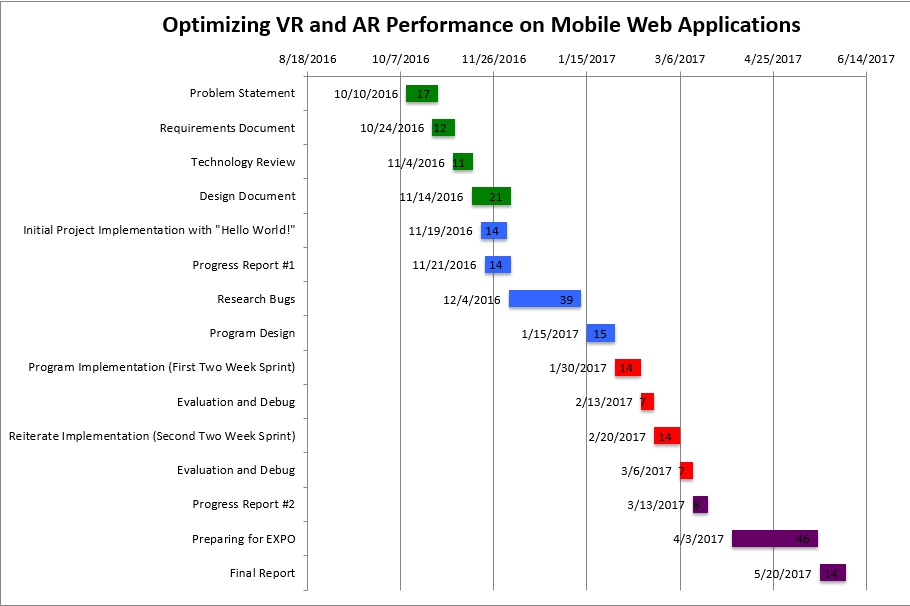
\includegraphics[width=6.5in]{OVRAR_Gantt_Chart.png}
    
\vfill
\noindent\begin{tabular}{ll}
\makebox[3.5in]{\hrulefill} & \makebox[1.5in]{\hrulefill}\\
Client Signature & Date\\
[4ex]% adds space between the two sets of signatures
\makebox[3.5in]{\hrulefill} & \makebox[1.5in]{\hrulefill}\\
Group Signature & Date\\
[4ex]% adds space between the two sets of signatures
\makebox[3.5in]{\hrulefill} & \makebox[1.5in]{\hrulefill}\\
Group Signature & Date\\
[4ex]% adds space between the two sets of signatures
\makebox[3.5in]{\hrulefill} & \makebox[1.5in]{\hrulefill}\\
Group Signature & Date\\
\end{tabular}
\end{document}